\section{Hybrid position/force control (HPFC)}

The goal of the snake robot is to push against obstacles in a fashion that yields forward propulsion along a path. Consequently, the robot will have to curve itself along the path whilst applying a force to the obstacles considered advantageous. The behavior of the robot has to comprise with the constraints arising from the contact, which further motivates the use of hybrid position/force control (HPFC).

HPFC is not a control method per se, but rather a method for determining when and in which directions force or motion control should be applied. It is desired to control motion along the unconstrained motion directions and force along the constrained motion directions. Different approaches to this problem exist. One is the use of selection matrices, introduced by Raibert and Craig et al. \cite{raibert1981hybrid}. The disadvantage of this approach is that the directions in which force and motion should be controlled has to be recalculated for every step, and is no simple procedure. In another approach, introduced by West and Asada \cite{west1985method}, two projection matrices are used as filters in joint space to automatically select between position- and force controlled vectors. There is however a disadvantage to this method as well, which is that the dynamics of the robot are ignored. A thoroughly studied method called dynamic HPFC, developed by Yoshikawa \cite{yoshikawa1987dynamic}, is therefore presented and adapted to the snake robot.

The theory on traditional HPFC up until the part \textit{Passive joints}, as well as this intro, is a modified part of the earlier project work of the author \cite{AtussaProsjektoppgp}. The rest of the chapter is focused on dynamic HPFC and the advantages and challenges that comes with adapting it to a snake robot model.

\subsection{Traditional HPFC} \label{subseq:HPFC}

Like mentioned above, velocity and force can be controlled in the directions in which they are not constrained. The end effector space of a robot can be divided into two orthogonal domains, a position domain and a force domain. These domains are complementary to the directions of the corresponding constraints at the end effector. It is logical to conclude that if there is contact with the environment, motion cannot be controlled freely. On the other hand, if there is no contact, there is no direction in which the robot can apply a force. Ergo, the force and motion control directions do not overlap and the domains are orthogonal. This means that position and force can be controlled independently and arbitrarily in these domains.

The following relationships are known from \ref{seq:constr_kin} and \ref{subseq:constr_dyn}. 

\begin{equation}
	\mathbf{v = J \dot{q}} \textrm{,} \quad  \  \boldsymbol{\tau} \mathbf{= J}^T \mathbf{f}
\end{equation}
\\
An important observation is that constraints due to contact with the environment are constraints due to a closed kinematic chain. In general, this is something that occurs when at least \textit{two} points of the robot are in contact with the environment. For the snake robot this might not always be the case. It is however possible to define a virtual closed kinematic chain where the robot is connected to the base with the virtual joint variables $x_0$, $y_0$ and $\phi_0$.
A separate Jacobian is calculated for each closed kinematic chain, as explained in \ref{subseq:constr_inst}.
%These Jacobians are denoted $\mathbf{J_{ci}}$, where $i = 1, .., k$ is the number of independent closed kinematic chains.
%Since the motion is constrained at a contact point, the relationships

Relationship (\ref{eq:constr_dyns}) comes from the motion being constrained at a contact point.

\begin{equation} \label{eq:constr_dyns}
    \mathbf{\dot{v}_{ci} = J_{ci} \dot{q} = 0}
\end{equation}
\\
The solution to (\ref{eq:constr_dyns}) can be proven to be

\begin{equation}
    \mathbf{\dot{q} = (I - J_{ci}^+ J_{ci}) y},
\end{equation}
\\
where $\mathbf{y}$ can be an arbitrary vector, as it will yield zero end effector motion. Furthermore, since the matrix $\mathbf{J_{ci}}$ might be non square, the pseudo inverse $\mathbf{J_{ci}^+}$ is used.
For a closed kinematic chain, the work done at the end of the chain must also be zero. Therefore, the sum of the work done by each of the joints must be zero:

\begin{equation} \label{eq:zero_joint_work}
    \boldsymbol{\tau^T} \mathbf{\dot{q}} = \boldsymbol{\tau^T} \mathbf{(I - J_{ci}^+ J_{ci}) y = 0}.
\end{equation}
\\
(\ref{eq:zero_joint_work}) has the general solution

\begin{equation}
   \boldsymbol{\tau}  \mathbf{= (J_{ci}^+ J_{ci})^T z},
\end{equation}
\\
where $\mathbf{z}$ can be an arbitrary vector.

The allowable motion is now characterized by $\mathbf{[I - J_{ci}^+ J_{ci}]}$ and the allowable forces by $\mathbf{[J_{ci}^+ J_{ci}]^T}$. These matrices are orthogonal projectors in joint space onto the allowable position and force variations respectively. A further explanation of this result is given in Chapter 5 of \cite{west1985method}. The projectors will be abbreviated to

\begin{equation}\label{eq:proj_mtrices}
    \prescript{}{j}{\mathbf{P}}_{ap} = \mathbf{[I - J_{ci}^+ J_{ci}]} \ \ \quad \textrm{and} \quad
    \prescript{}{j}{\mathbf{P}}_{af} = \mathbf{[J_{ci}^+ J_{ci}]^T = [I - (\prescript{j}{ap}{P})^T]}.
\end{equation}
\\
The subscript $j$ denotes joint space, and $ap$ and $af$ stand for allowable positions and allowable forces respectively. It can be observed that these projection matrices project onto the nullspace of the respective constraint directions. This can further be related to the concept of task priority, in which tasks with lower priority are performed in the null-space of higher priority tasks \cite{chiaverini2008kinematically}. An important observation is that the mapping onto the allowable force and position spaces are in this method purely determined by the kinematics of the robot.

\subsubsection{Multiple constraints}\label{subseq:mult_contacts}

If there are several contact points, projection matrices are calculated for each constraint, and the final projection matrices are found by taking the union and intersect of the different $\prescript{}{j}{\mathbf{P}}_{af}$ and $\prescript{}{j}{\mathbf{P}}_{ap}$ respectively.

\subsubsection{Passive joints}

The presence of passive joints in the robot imposes another constraint on the allowable forces. This is because the force in a passive joint is uncontrollable. \cite{west1985method} presents two methods of including this constraint. One of which is using a diagonal matrix $\mathbf{A}$ that denotes which joints are passive and which are active. A 1 on the diagonal indicates an active joint whereas a 0 indicates a passive joint. This matrix has to be manually initialized before controlling the robot. It can then be combined with the allowable force projection by taking the intersect of the space spanned by $\mathbf{A}$ and $\prescript{}{j}{\mathbf{P}}_{af}$.

\subsubsection{Task analysis}

An end effector task may consist of both a movement and force application onto a surface. The projectors $\prescript{}{j}{\mathbf{P}}_{ap}$ and $\prescript{}{j}{\mathbf{P}}_{af}$ make sure the force and movement are performed in the allowable force and movement directions. A specific task may however not be possible to perform within the restrictions of these spaces.

\textit{Essential position variables} are defined as the directions om movement of the end effector which must be controlled in order to perform the task correctly. At the same time, \textit{arbitrary position variables} are those directions of movement which do not have to be controlled precisely. The terms \textit{essential force variables} and \textit{arbitrary force variables} follow the same logic, just for the force directions. According to \cite{west1985method}, the total number of essential variables, position plus force, is equal to the minimum number of controllable actuators in the manipulator necessary for performing the task.

The essential position and force direction can be described by the column vectors (\ref{eq:hpfc_ep}) and (\ref{eq:hpfc_ef}) respectively.

\begin{equation}\label{eq:hpfc_ep}
    \mathbf{E}_p =
    \begin{bmatrix}
        \mathbf{e}_{p1} & ... & \mathbf{e}_{p\alpha}
    \end{bmatrix}^T
\end{equation}

\begin{equation}\label{eq:hpfc_ef}
    \mathbf{E}_f =
    \begin{bmatrix}
        \mathbf{e}_{f1} & ... & \mathbf{e}_{f\beta}
    \end{bmatrix}^T
\end{equation}
\\
Each column vector describes one direction. Following, the number of essential position directions is $\alpha$ and the number of essential force directions is $\beta$. The orthogonal projections onto the essential position and force spaces are given by (\ref{eq:hpfc_wep}) and (\ref{eq:hpfc_wef}) respectively.

\begin{equation}\label{eq:hpfc_wep}
    \prescript{}{w}{\mathbf{P}}_{ep} = \mathbf{E}_p(\mathbf{E}_p^T \mathbf{E}_p)^{-1} \mathbf{E}_p^T
\end{equation}

\begin{equation}\label{eq:hpfc_wef}
    \prescript{}{w}{\mathbf{P}}_{ef} = \mathbf{E}_f(\mathbf{E}_f^T \mathbf{E}_f)^{-1} \mathbf{E}_f^T
\end{equation}
\\
The inverse in the two equations above is, probably by mistake, not included in \cite{west1985method}. The $w$ denotes that the projectors are defined in work space coordinates. In order to combine these projectors with the allowable position and force projectors, it is desirable to define them in the joint space coordinate system. The precondition for this to be possible for the essential position space is that the number of joints linking the base of the manipulator to the end effector is greater than or equal to three (given the two dimensional case). For the essential force space, the number of \textit{active} joints has to be greater than or equal to three. The joint space projectors can then be found by

\begin{equation}\label{eq:hpfc_jep}
    \prescript{}{j}{\mathbf{P}}_{ep} = \mathbf{J}_t^+ \prescript{}{w}{\mathbf{P}}_{ep} \mathbf{J}_t
\end{equation}

\begin{equation}\label{eq:hpfc_jeF}
    \prescript{}{j}{\mathbf{P}}_{ef} = \mathbf{J}_c^+ \prescript{}{w}{\mathbf{P}}_{ef} (\mathbf{J}_c^T)^+
\end{equation}
\\
The Jacobian $\mathbf{J}_t$ relates the task specific coordinates to the joint space. Section \ref{subsec:DHPFC} explains how this Jacobian can be found for the snake robot case.

Eventually, the projections in joint space that project onto the allowable motion and force spaces \textit{and} result in the desired motion and force necessary to perform the task are given by (\ref{eq:hpfc_fp}) and (\ref{eq:hpfc_ff}) respectively.

\begin{equation}\label{eq:hpfc_fp}
    \prescript{}{j}{\mathbf{F}}_{p} = \prescript{}{j}{\mathbf{P}}_{ap} (\prescript{}{j}{\mathbf{P}}_{ep} \prescript{}{j}{\mathbf{P}}_{ap})^+ \prescript{}{j}{\mathbf{P}}_{ep}
\end{equation}

\begin{equation}\label{eq:hpfc_ff}
    \prescript{}{j}{\mathbf{F}}_{f} = \prescript{}{j}{\mathbf{P}}_{af} (\prescript{}{j}{\mathbf{P}}_{ef} \prescript{}{j}{\mathbf{P}}_{af})^+ \prescript{}{j}{\mathbf{P}}_{ef}
\end{equation}

\subsection{Dynamic HPFC} \label{subsec:DHPFC}

The solution of West and Asada \cite{west1985method} does not take the manipulator dynamics into account. Nevertheless, in a real system, the dynamics play a significant role in the resulting behavior of the robot. For this reason, Yoshikawa \cite{yoshikawa1987dynamic} designed the dynamic hybrid control method which incorporates the constraints into the manipulator dynamics. More specifically, the solution of \cite{west1985method} filters the commanded joint torques and angles to conform to the constraints. These filters are, as described in \ref{subseq:HPFC}, based on the kinematic Jacobian of the system. The essence of the solution of \cite{yoshikawa1987dynamic} however, is that the robot dynamics and constraint equations are combined before the commanded torques and angles are calculated. 

This section aims at describing the improved method, and the content is based the paper of \cite{yoshikawa1987dynamic}. The symbolic conventions used are for simplicity the same as in the paper. The next section will explain further how the theory and these symbols apply to the snake robot case and the snake robot specific theory presented earlier in this chapter \hl{ref this}.

It is worth noting that the solution of Yoshikawa is designed for a robot manipulator with a static base where the only constraint present is targeted at the manipulator end effector. For this reason, special effort has been put into finding a suitable formulation of the snake robot constraints. Additionally, the difference between the coordinate spaces introduced in the paper are easy to confuse and special attention has been directed at thoroughly defining these spaces for the snake robot so that the following calculations can be both as clear and logical as possible.

\begin{figure}
    \centering
    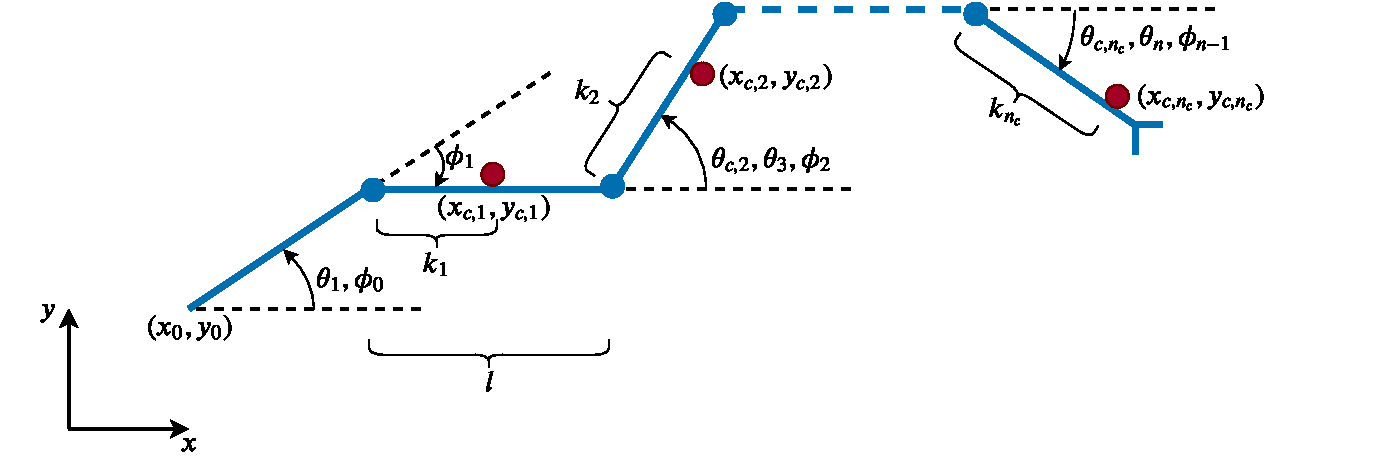
\includegraphics[width=\textwidth]{figures/theory/dhpfc_robot.pdf}
    \caption{Model of snake robot and obstacles illustrating joint and obstacle variables}
    \label{fig:dhpfc_robot1}
\end{figure}
\begin{figure}
    \centering
    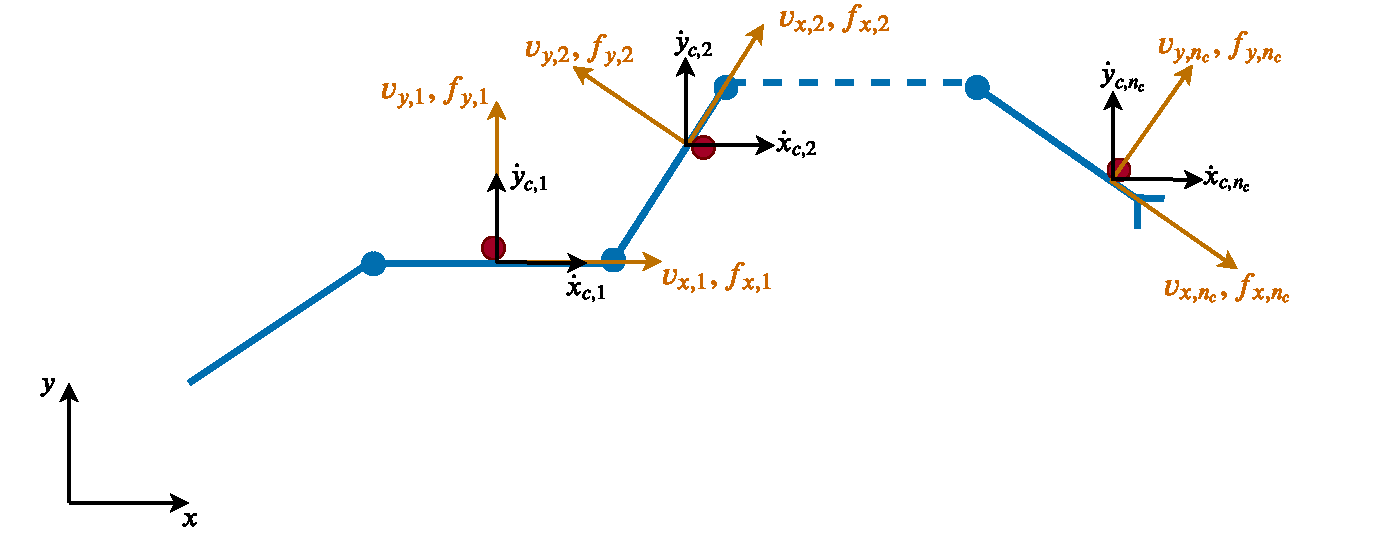
\includegraphics[width=\textwidth]{figures/theory/dhpfc_robot_2.pdf}
    \caption{Model of snake robot and obstacles illustrating velocity and force directions}
    \label{fig:dhpfc_robot2}
\end{figure}

\subsubsection{Description of constraints}

In order to take the dynamics into account, the constraints are directly included into the dynamic equations of motion of the robot. This is done by expressing the constraints as a set of hypersurfaces that the robot can not physically pass. It should be noted that the focus here is on manipulator end-effector constraints and not general constraints which should be used in the snake robot case. The constraint hypersurfaces are also expressed in the end-effector coordinates. Another important aspect of the paper is that it only addresses bilateral hypersurfaces (and not unilateral surfaces), meaning that the effector is prohibited from leaving the surface in any direction.

It is assumed that a given constraint can be expressed by a set of $m$ hypersurfaces

\begin{equation}\label{eq:hpfc:hypersurface}
    p_i(\mathbf{r}) = 0, \quad i = 1, 2, ..., m,
\end{equation}
\\
where $\mathbf{r}$ is the end effector position in a fixed reference frame. Differentiating (\ref{eq:hpfc:hypersurface}) with respect to time yields

\begin{equation}\label{eq:hpfc:derhypsurf}
    \mathbf{E}_F \mathbf{\dot{r}} = 0,
\end{equation}
\\
where the vectors of $\mathbf{E}_F$ are the unit normal vectors to the hypersurfaces in (\ref{eq:hpfc:hypersurface}).

By comparing the expression (\ref{eq:norm_vel4}) of the constraint on link $i$ found in \ref{seq:constraints} to (\ref{eq:hpfc:derhypsurf}), it is possible to extract the matrix $\mathbf{E}_{F,i}$ and a logical choice of $\mathbf{r}_i$ and $\mathbf{\dot{r}}_i$ presents itself.
Specifically, if one chooses

\begin{equation}
    \mathbf{r}_i =
    \begin{bmatrix}
        x_{c,i} & y_{c,i} & \theta_{c,i}
    \end{bmatrix}^T \in \mathcal{R}^3,
\end{equation}
\\
then $\mathbf{\dot{r}}_i = [\dot{x}_{c,i}, \dot{y}_{c,i}, \dot{\theta}_{c,i}]^T \in \mathcal{R}^3$ and the matrix $\mathbf{E}_{F,i}$ can by comparison be found as

\begin{equation}
    \mathbf{E}_{F,i} =
    \begin{bmatrix}
        -sin(\theta_{c,i}) & cos(\theta_{c,i}) & 0
    \end{bmatrix} \in \mathcal{R}^3.
\end{equation}
\\
The subscript $i$ will now be used as the constraint number, where $n_c$ is the number of constraints/contact points.
The angle of the link at the contact point $\theta_{c,i}$ with respect to the base frame is the same as the angle $\theta$ of the link in contact with respect to the base frame. It can by inspection be seen that $\mathbf{E}_{F,i}$ fulfills the criteria of being of unit size.

These formulations do not supply an explicit expression of the corresponding constraint hypersurface. It is however not a necessity for the further computations. On the other hand it could be valuable to have the expressions for the hypersurfaces for analysis purposes.

The coordinate space $\mathbf{r}$ should be able to aid in expressing all the constraints present on the snake robot. Therefore, it is chosen as 

\begin{equation}
    \mathbf{r} = 
    \begin{bmatrix}
        \mathbf{r}_1^T & \mathbf{r}_2^T & \dots &\mathbf{r}_{n_c}^T
    \end{bmatrix}^T \in \mathcal{R}^{3 n_c}.
\end{equation}
\\
The same goes for $\dot{\mathbf{r}}$. Furthermore, the matrix $\mathbf{E}_{F}$ describing the unit normal vectors to all the hypersurfaces can now be written as

\begin{equation}
    \mathbf{E}_F = 
    \begin{bmatrix}
        \mathbf{E}_{F,1} & \mathbf{0}_{1\times3} & \dots & \mathbf{0}_{1\times3} \\
        \mathbf{0}_{1\times3} & \ddots & & \vdots \\
        \vdots & & \ddots & \mathbf{0}_{1\times3} \\
        \mathbf{0}_{1\times3} & \dots & \mathbf{0}_{1\times3} & \mathbf{E}_{F,n_c} \\
    \end{bmatrix} \in \mathcal{R}^{n_c \times 3 n_c}
\end{equation}
\\

Differentiating (\ref{eq:hpfc:derhypsurf}) further gives

\begin{equation}\label{eq:dhpfc_arf}
    \mathbf{E}_F \mathbf{\ddot{r}} + \mathbf{a}_{r F} = 0, \quad \mathbf{a}_{r F} = \mathbf{\dot{E}}_F\mathbf{\dot{r}}
\end{equation}
\\
For the snake robot case $\mathbf{a}_{r F} \in \mathcal{R}^{n_c}$.

Furthermore, $\mathbf{E}_P$ is chosen so that all the vectors in the relation

\begin{equation}\label{eq:dhpfc_E}
    \mathbf{E} =
    \begin{bmatrix}
    \mathbf{E}_P \\ \mathbf{E}_F
    \end{bmatrix}
\end{equation}
\\
are mutually independent unit vectors. The matrix $\mathbf{E}_F$ represents the coordinate axes normal to the constraint surfaces, and $\mathbf{E}_P$ represents the coordinate axes complementing $\mathbf{E}_F$. Another way to display this is seeing $\mathbf{E}_F$ and $\mathbf{E}_P$ as the axes for force and position constrained directions respectively.

From the equations

\begin{equation}
    \mathbf{E\dot{r}} =
    \begin{bmatrix}
        \mathbf{E}_P \mathbf{\dot{r}}\\
        0
    \end{bmatrix}
    \quad \text{and} \quad
    \mathbf{E\ddot{r}} =
    \begin{bmatrix}
        \mathbf{E}_P \mathbf{\ddot{r}} \\
        -\mathbf{a}_{r F}
    \end{bmatrix}
\end{equation}
\\
it can be seen that the velocity to the constraint surface is zero, which is natural seeing as the end-effector should be physically unable to move through the surface.

For the snake robot, a simple choice of $\mathbf{E}_{P,i}$ with unit vectors complementing $\mathbf{E}_{F,i}$ is by inspection found to be

\begin{equation}\label{eq:dhpfc_EPi}
    \mathbf{E}_{P,i} = 
    \begin{bmatrix}
        cos(\theta_{c,i}) & sin(\theta_{c,i}) & 0 \\
        0 & 0 & 1
    \end{bmatrix} in \mathcal{R}^{2\times 3}.
\end{equation}
\\
Again, $\mathbf{E}_{P,i}$ corresponds to the $i$'th constraint. Combining all $\mathbf{E}_{P,i}$ gives 

\begin{equation}
    \mathbf{E}_P = 
    \begin{bmatrix}
        \mathbf{E}_{P,1} & \mathbf{0}_{2\times3} & \dots & \mathbf{0}_{2\times3} \\
        \mathbf{0}_{2\times3} & \ddots & & \vdots \\
        \vdots & & \ddots & \mathbf{0}_{2\times3} \\
        \mathbf{0}_{2\times3} & \dots & \mathbf{0}_{2\times3} & \mathbf{E}_{P,n_c} \\
    \end{bmatrix} \in \mathcal{R}^{2 n_c \times 3 n_c}
\end{equation}
\\
and $\mathbf{E} \in \mathcal{R}^{3 n_c \times 3 n_c}$.

%%%%%%%%%%%%%%%%%%%%%%%%%%%%%%%%%%%%%%%%%%%%%%%%%%%%%%%%%%%%%%%%%%%%%%%%%%%%%%%%%%%%%%%%%%%%%
%%%%%%%%%%%%%%%%%%%%%%%%%%%%%%%%%%%%%%%%%%%%%%%%%%%%%%%%%%%%%%%%%%%%%%%%%%%%%%%%%%%%%%%%%%%%%
%%%%%%%%%%%%%%%%%%%%%%%%%%%%%%%%%%%%%%%%%%%%%%%%%%%%%%%%%%%%%%%%%%%%%%%%%%%%%%%%%%%%%%%%%%%%%

\subsubsection{Kinematics and dynamics}

In \cite{yoshikawa1987dynamic}, the relation between the joint variable vector $\mathbf{q}$ and the end effector position $\mathbf{r}$ is expressed as

\begin{equation}\label{eq:hpfc:rq}
    \mathbf{r = c(q)}.
\end{equation}
\\
The following equations are generated by differentiating \ref{eq:hpfc:rq}.

\begin{equation}
    \mathbf{\dot{r} = J \dot{q}}, \quad \mathbf{J} = \frac{\partial \mathbf{c(q)}}{\partial \mathbf{q}^T}
\end{equation}

\begin{equation}\label{eq:dhpfc_aq}
    \mathbf{\ddot{r} = J \ddot{q}} + \mathbf{a}_q, \quad \mathbf{a}_q = \mathbf{\dot{J} \dot{q}}   
\end{equation}
\\
For the snake robot case, the matrix $\mathbf{J}$ is the Jacobians of all the contacts/constraints.

\begin{equation}
    \mathbf{J} = 
    \begin{bmatrix}
        \mathbf{J}_1 \\ \mathbf{J}_2 \\ \vdots \\ \mathbf{J}_{n_c}
    \end{bmatrix} \in \mathcal{R}^{3 n_c \times N}
\end{equation}
\\
$N$ is from section \ref{sec:kin} known as the size of $\mathbf{q}$. The Jacobian is also explained in the mentioned section. The Jacobian $\mathbf{J}_i \in \mathcal{R}^{3\times N}$ for a single contact point with respect to the contact point variable vector $\mathbf{r}_i$ is found as 

\begin{equation}
    \mathbf{J}_i =
    \HUGE{
    \begin{bmatrix}
        \frac{\partial x_{c,i}}{\partial q_1} & \dots & \frac{\partial x_{c,i}}{\partial q_N} \\
        \frac{\partial y_{c,i}}{\partial q_1} & \dots & \frac{\partial y_{c,i}}{\partial q_N} \\
        \frac{\partial \theta_{c,i}}{\partial q_1} & \dots & \frac{\partial \theta_{c,i}}{\partial q_N}
    \end{bmatrix}
    }.
\end{equation}
\\
Furthermore, $\mathbf{a}_q \in \mathcal{R}^{n_c}$.


The relationship between the velocity vector $\mathbf{v}$ given in the end effector frame and the velocity vector $\dot{\mathbf{r}}$ in the fixed reference frame is given by the transformation matrix $\mathbf{T}$ in (\ref{eq:hpfc:vTr}).
\begin{equation}\label{eq:hpfc:vTr}
    \mathbf{v = T\dot{r}}
\end{equation}
\\
The interpretation of this velocity vector for the snake robot case is
\begin{equation}
    \mathbf{v}_i = 
    \begin{bmatrix}
        v_{x,i} & v_{y,i}
    \end{bmatrix}^T \in \mathcal{R}^2.
\end{equation}
This is the velocity of the $i$'th contact point given in the coordinate frame of the contact point. This is better explained by the illustration in Figure \ref{}.

The corresponding transformation matrix converting between $\mathbf{r}_i$ and $\mathbf{v}_i$ is

\begin{equation} \label{eq:dhpfc_Ti}
    \mathbf{T}_i =
    \begin{bmatrix}
        cos(\theta_{c,i}) & sin(\theta_{c,i}) & 0 \\
        -sin(\theta_{c,i}) & cos(\theta_{c,i}) & 0
    \end{bmatrix} \in \mathcal{R}^{2 \times 3},
\end{equation}
\\
which is simply a rotation around the local z-axis. Its inverse is given by

\begin{equation}\label{eq:Tinv}
    \mathbf{T}^{-1}_i =
    \begin{bmatrix}
        cos(\theta_{c,i}) & -sin(\theta_{c,i}) \\
        sin(\theta_{c,i}) & cos(\theta_{c,i}) \\
        0 & 0
    \end{bmatrix} \in \mathcal{R}^{3 \times 2}.
\end{equation}
\\
Combining all the transformation matrices yields

\begin{equation}
    \mathbf{T} =
    \begin{bmatrix}
        \mathbf{T}_1 & \mathbf{0}_{2\times3} & \dots & \mathbf{0}_{2\times3} \\
        \mathbf{0}_{2\times3} & \ddots & & \vdots \\
        \vdots & & \ddots & \mathbf{0}_{2\times3} \\
        \mathbf{0}_{2\times3} & \dots & \mathbf{0}_{2\times3} & \mathbf{T}_{n_c} \\
    \end{bmatrix} \in \mathcal{R}^{2 n_c \times 3 n_c}
\end{equation}
\\

From (\ref{eq:hpfc:derhypsurf}) and (\ref{eq:hpfc:vTr}) it follows that

\begin{equation}\label{eq:hpfc:EFTv}
    \mathbf{E}_F \mathbf{T}^{-1} \mathbf{v} = 0.
\end{equation}
\\
Furthermore, it is assumed that no friction works between the constraint surface and the end-effector. Thus, from the principle of virtual work, the force $\mathbf{f}$ exerted on the surface by the effector must follow

\begin{equation}\label{eq:hpfc:vf}
    \mathbf{v}^T \mathbf{f} = 0.
\end{equation}
\\
An interpretation is, like mentioned above, that the force and velocity directions complement each other. From (\ref{eq:hpfc:EFTv}) and (\ref{eq:hpfc:vf}) it follows that

\begin{equation}
    \mathbf{f} = \hat{\mathbf{E}}_F^T \mathbf{f}_F, \quad \hat{\mathbf{E}}_F^T = \mathbf{E}_F \mathbf{T}^{-1},
\end{equation}
\\
where $\mathbf{f}_F$ is an unknown vector representing the force $\mathbf{f}$ in terms of the unit force vectors.

Calculating the force $\mathbf{f}_i$ for a given contact point gives

\begin{equation}
    \begin{split}
        \mathbf{f}_i &= \hat{\mathbf{E}}_{F,i}^T \mathbf{f}_{F,i} = \mathbf{E}_{F,i} \mathbf{T}_i^{-1} \mathbf{f}_{F,i}\\
        &=
        \begin{bmatrix}
            -sin(\theta_{c,i}) & cos(\theta_{c,i}) & 0
        \end{bmatrix}
        \begin{bmatrix}
            cos(\theta_{c,i}) & -sin(\theta_{c,i}) \\
            sin(\theta_{c,i}) & cos(\theta_{c,i}) \\
            0 & 0
        \end{bmatrix}
        \mathbf{f}_{F,i}\\
        &=
        \begin{bmatrix}
            0 \\ 1
        \end{bmatrix}
        \mathbf{f}_{F,i}
    \end{split}
\end{equation}
\\
This result corresponds with the intuition gained from studying figure \ref{}. \hl{Write some more about this result.}

The corresponding torque is found by

\begin{equation}
    \boldsymbol{\tau}_F = (\mathbf{TJ})^T \mathbf{f} = \mathbf{J}^T \mathbf{E}_F^T \mathbf{f}_F.
\end{equation}

%%%%%%%%%%%%%%%%%%%%%%%%%%%%%%%%%%%%%%%%%%%%%%%%%%%%%%%%%%%%%%%%%%%%%%%%%%%%%%%%%%%%%%%%%%%%%
%%%%%%%%%%%%%%%%%%%%%%%%%%%%%%%%%%%%%%%%%%%%%%%%%%%%%%%%%%%%%%%%%%%%%%%%%%%%%%%%%%%%%%%%%%%%%
%%%%%%%%%%%%%%%%%%%%%%%%%%%%%%%%%%%%%%%%%%%%%%%%%%%%%%%%%%%%%%%%%%%%%%%%%%%%%%%%%%%%%%%%%%%%%

\subsubsection{Calculation of the joint driving force}

The total torque $\boldsymbol{\tau}$ applied to the robot will be the difference between the motor torque $\boldsymbol{\tau}_c$ and the constraint torque $\boldsymbol{\tau}_F$.

\begin{equation}\label{eq:tau_dhpfc1}
    \boldsymbol{\tau} = \boldsymbol{\tau}_c - \boldsymbol{\tau}_F
\end{equation}
\\

Combining the torque in (\ref{eq:tau_dhpfc1}) with the equations of motion given in (\ref{eq:eom}) gives

\begin{equation}\label{eq:dhpfc_stuff1}
    \mathbf{M(q) \ddot{q}} + \mathbf{J}^T \mathbf{E}^T_F \mathbf{f}_F = \boldsymbol{\tau}_c - \mathbf{C(q, \dot{q})}
\end{equation}
\\
and
\begin{equation}\label{eq:dhpfc_stuff2}
    \mathbf{E}_F \mathbf{J\ddot{q}} = - \mathbf{E}_F \mathbf{a}_q - \mathbf{a}_{rF}.
\end{equation}
\\
Lastly, it can be shown that combining (\ref{eq:dhpfc_stuff1}) and (\ref{eq:dhpfc_stuff2}) yields the expressions

\begin{equation}
    \mathbf{\ddot{q}} = \mathbf{M}^{-1}(\mathbf{b}_1 + (\mathbf{E}_F \mathbf{J})^T \mathbf{K} (\mathbf{b}_2 - \mathbf{E}_F \mathbf{J} \mathbf{M}^{-1} \mathbf{b}_1)),
\end{equation}

\begin{equation}
    \mathbf{f}_F = -\mathbf{K} (\mathbf{b}_2 - \mathbf{E}_F \mathbf{J} \mathbf{M}^{-1} \mathbf{b}_1).
\end{equation}
\\
$\mathbf{K}$, $\mathbf{b}_1$ and $\mathbf{b}_2$ are given by

\begin{equation}
    \begin{split}
        \mathbf{K} &= (\mathbf{E}_F \mathbf{J} \mathbf{M}^{-1} \mathbf{J}^T \mathbf{E}^T_F)^{-1}\\
        \mathbf{b}_1 &= \boldsymbol{\tau}_c - \mathbf{C(q, \dot{q})}\\
        \mathbf{b}_2 &= - \mathbf{E}_F \mathbf{a}_q - \mathbf{a}_{rF}.
    \end{split}
\end{equation}
\\
Eventually, it is possible to calculate the joint control torque. It consists of a component based on the desired movement $\mathbf{\ddot{r}}_d$ and a component based on the desired force $\mathbf{f}_{Fd}$ at applied to the constraint surfaces.

\begin{equation}\label{eq:dhpfc_tau_c}
    \boldsymbol{\tau}_c = \boldsymbol{\tau}_P + \boldsymbol{\tau}_F
\end{equation}
\\
The torque $\boldsymbol{\tau}_P$ is found by solving the equations of motion given in (\ref{eq:eom}) based on the desired values of the joint accelerations.

\begin{equation}
    \boldsymbol{\tau}_P = \mathbf{M(q)} \ddot{\mathbf{q}}_d + \mathbf{C}(\mathbf{q,\dot{q}})
\end{equation}

\begin{equation}
    \boldsymbol{\tau}_F = \mathbf{J}^T \mathbf{E}^T_F \mathbf{f}_{Fd}
\end{equation}

\begin{equation}\label{eq:dhpfc_qddd}
    \ddot{\mathbf{q}}_d = \mathbf{J}^+ (\mathbf{E}^{-1} 
    \begin{bmatrix}
        \mathbf{\ddot{r}}_{EPd} \\
        - \mathbf{a}_{rF}
    \end{bmatrix}
    - \mathbf{a}_q)
\end{equation}
\\
Here the vector $\mathbf{\ddot{r}}_{EPd} = \mathbf{E}_P \mathbf{\ddot{r}}_{d}$. Furthermore, $\mathbf{J}^+$ denotes the pseudo inverse of the Jacobian. According to Yoshikawa \cite{yoshikawa1987dynamic} the position and force can be simultaneously controlled by applying the sum of the joint torque $\boldsymbol{\tau}_P$ for achieving the desired acceleration and the joint torque $\boldsymbol{\tau}_F$ for achieving the desired force as long as the robot is not in a singular state.

Describing the desired acceleration through $\mathbf{\ddot{r}}_d$ might not be the most intuitive task. It is therefore suggested that $\mathbf{E}_P$ is chosen in such a manner that a function $\mathbf{\dot{r}}_P = s(\mathbf{r})$ exists and satisfies

\begin{equation}
    \mathbf{\dot{r}}_P = \mathbf{E}_P \mathbf{\dot{r}}.
\end{equation}
\\
If this holds, then
\begin{equation}
    \mathbf{\ddot{r}}_P = \mathbf{\ddot{r}}_{EP} + \mathbf{a}_{rP}, \quad \mathbf{a}_{rP} = \mathbf{\dot{E}}_P \mathbf{\dot{r}}_P.
\end{equation}
\\
Given that $\mathbf{r}_{P}$ is given by $\mathbf{r}_{Pd}$ and the described dynamics and constraints are correct, the system given by (\ref{eq:dhpfc_tau_c})-(\ref{eq:dhpfc_qddd}) will be able to realize both the desired position and force.


%%%%%%%%%%%%%%%%%%%%%%%%%%%%%%%%%%%%%%%%%%%%%%%%%%%%%%%%%%%%%%%%%%%%%%%%%%%%%%%%%%%%%%%%%%%%%
%%%%%%%%%%%%%%%%%%%%%%%%%%%%%%%%%%%%%%%%%%%%%%%%%%%%%%%%%%%%%%%%%%%%%%%%%%%%%%%%%%%%%%%%%%%%%
%%%%%%%%%%%%%%%%%%%%%%%%%%%%%%%%%%%%%%%%%%%%%%%%%%%%%%%%%%%%%%%%%%%%%%%%%%%%%%%%%%%%%%%%%%%%%

\subsection{The benefits of dynamic HPFC in snake robot locomotion}

Give a brief overview of the most important strategies for terrestrial snake robot locomotion, and
discuss the prospective properties of HPFC in the context of your findings.

- Controlling both the force and position using compliance control would require us to frequently switch between very very high and very low compliance. Det er vel directional compliance tho

- vi likevel ha en viss compliant behavior i at hvis en hindring beveger seg litt vil slangen følge etter --> men det kan være en assumption at hindringene har statisk posisjon

- Lateral undulation etc is optimal for flat, obstacle-free environments. HPFC is useless in this case

- Allows us to control force and position simultaneously in different directions.

- posisjonsstyring gir stiv oppførsel og krafstyring gir dynamisk oppførsel

%%%%%%%%%%%%%%%%%%%%%%%%%%%%%%%%%%%%%%%%%%%%%%%%%%%%%%%%%%%%%%%%%%%%%%%%%%%%%%%%%%%%%%%%%%%%%
%%%%%%%%%%%%%%%%%%%%%%%%%%%%%%%%%%%%%%%%%%%%%%%%%%%%%%%%%%%%%%%%%%%%%%%%%%%%%%%%%%%%%%%%%%%%%
%%%%%%%%%%%%%%%%%%%%%%%%%%%%%%%%%%%%%%%%%%%%%%%%%%%%%%%%%%%%%%%%%%%%%%%%%%%%%%%%%%%%%%%%%%%%%

\subsection{The challenges related to the application of dynamic HPFC}

There are surely several ways of implementing and designing the dynamic HPFC control logic on a snake robot. This section will focus on the challenges related to the application of the suggested design scheme in \ref{subsec:DHPFC}. Special attention is paid to the chosen variable spaces and the consequences of configuration transitions when the snake moves.

\subsubsection{Computational challenges}

Whenever the snake achieves successful forward or backward propulsion it will slide along the obstacles that are by its side. Eventually the contact between a link and an obstacle will be lost. At this point, the obstacle will either be left alone or come in contact with a neighboring link. These two scenarios are illustrated in Figures \ref{fig:obst_slide_seq1} and \ref{fig:obst_slide_seq2} respectively. If the contact is completely lost, it means that one constraint is lost as well and $n_c = n_c - 1$. This will in turn lead to the variable $\mathbf{r}$, describing the position of the contacts, shrinking. Consequently the mapping matrix $\mathbf{E}$ to the allowed force and movement directions will shrink as well. The greatest challenge in this case is changing the dimensions of the relevant variables in real time. One option could however be keeping all variable spaces and instead set the parts of $\mathbf{E}$ corresponding to the lost constraint to zero so that it has no impact on the following solution.

\begin{figure}
    \centering
    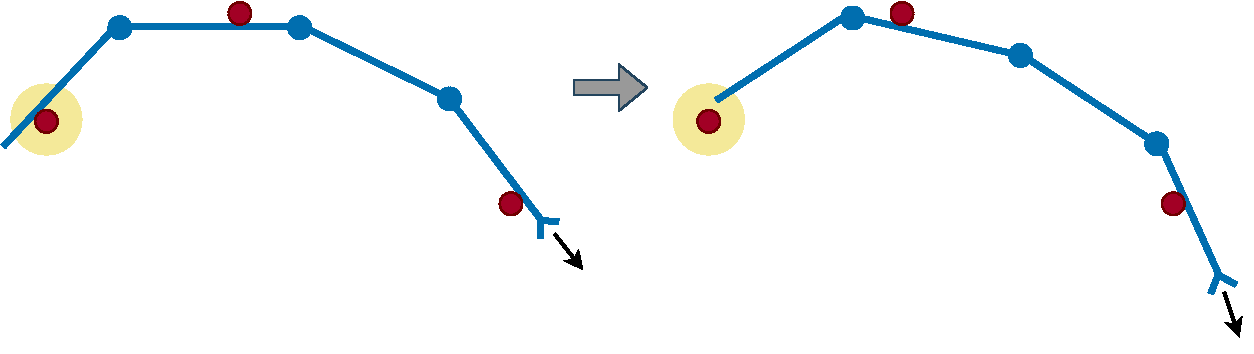
\includegraphics[width=\textwidth]{figures/theory/obst_slide_sequence1.pdf}
    \caption{Snake robot losing contact with obstacle}
    \label{fig:obst_slide_seq1}
\end{figure}

\begin{figure}
    \centering
    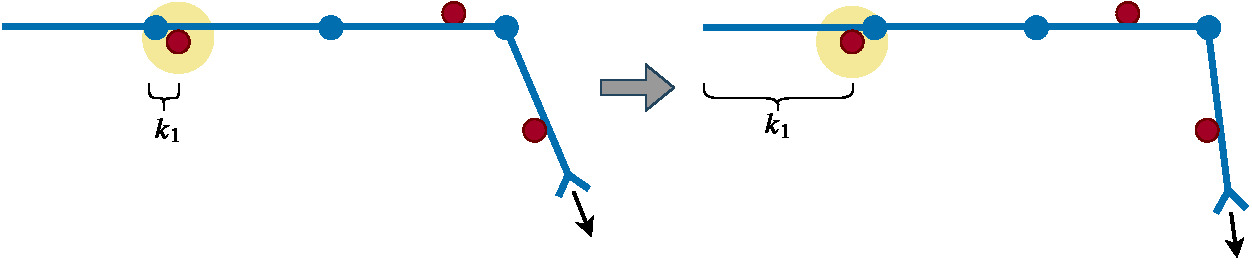
\includegraphics[width=\textwidth]{figures/theory/obst_slide_sequence2.pdf}
    \caption{Obstacle changing contact from one link to another}
    \label{fig:obst_slide_seq2}
\end{figure}

If, on the other hand, the snake simply slides in a way that the contact is transferred to an adjoining link, the size $n_c$ and dimensions of all variables will remain unchanged. In addition to this, the obstacle will lie on the same side of the snake as it already was, which enables the direction of the desired force application to the obstacle to stay the same as well. Thus, the constraint will generally be on the same form. The only thing that has to change is the description of the position variables in $\mathbf{r}$ belonging to the new contact point. Again, the change is most probably slim since the two first variables $(x_c, y_c)$ describe the position of the contact point and the obstacle is assumed to be static (meaning its position will not change). Furthermore, the adjoining link adopting the contact is probable to have a similar angle $\theta_c = \theta$ relative to the base frame as the previous link given that the desired path is well designed and defined. This obviously makes the implementation simpler and the control sequence smoother and more predictable.

Even though the magnitude of the mentioned variables do not change drastically, the Jacobian will have to be recalculated since the variables now are described by a new subset of the joint variables. Finding a new expression for the Jacobian matrix and its derivative in real time is not a trivial, nor fast, operation. One option would of course be pre-computing $\mathbf{J}$ and $\dot{\mathbf{J}}$ for every link that could be in contact with an obstacle and only employ the ones that are relevant at the specific time instance. There is however still a challenge related to this case. The generalized joint variables $\mathbf{q}$ contain the distances $k$ from the contact points to the preceding joints. It is important that these distances are not mixed and that they are only used once. In other words, two contact points should not be described by the same $k$. As a consequence of this, the Jacobian for every link would have to be computed with all the possible $k$'s. Logically, this would in turn lead to a large number of pre-computed matrices as the number of links and obstacles grow. In addition to this, the right set of Jacobians would have to be chosen real time while administering that they all use unique $k$'s. This should be done without changing the existing setup more than necessary in order to avoid jumps in the control. It is very much an achievable task, but at the same time an extra challenge.

With a contact moving from one link to another, the corresponding joint variable $k$ describing the position of the contact point will change and the manner in which it is computed will change as well. This is once again an achievable, yet challenging task to perform in real-time. It should also be noted that the value of this $k$ will probably experience a jump. This is because the contact moves from the end of a link to the beginning of a link, or vice versa, and the distance is always measured with respect to the preceding joint of the link in contact. This is illustrated in Figure \ref{fig:obst_slide_seq2}. On the other hand, it is reassuring that the matrices $\mathbf{M(q)}$ and $\mathbf{C(q,\dot{q})}$ are unaltered by the change of a $k$. This is logical since these matrices describe the dynamics of the snake robot alone.

The greatest challenge arises if the number of contact points increase. This means that the dimension of all variables will have to increase correspondingly and the Jacobians have to be either re-computed or re-assembled. It is in this case important to keep in mind the challenge associated with memory allocation in the software being used.

\subsubsection{Differences with the traditional manipulator case}

- Not actuation in all joints / all degrees of freedom (some are uncontrollable)

- Arbitrary number of obstacles and constantly changing requirements (desired force application etc, as opposed to a typical industrial manipulator that simply should polish a surface with a given pressure repeatedly)

- The environment is constantly changing and the contact wont be a point contact in the real world, and the snake robot might encounter all kinds of surfaces and textures (rigid, soft, slippery etc)

\subsubsection{Utilizing the force and position spaces}

Pay special attention to the
roles played by the so-called force and position spaces, and how these can be utilized and further
decomposed to illuminate necessary and sufficient conditions for propulsion.

%%%%%%%%%%%%%%%%%%%%%%%%%%%%%%%%%%%%%%%%%%%%%%%%%%%%%%%%%%%%%%%%%%%%%%%%%%%%%%%%%%%%%%%%%%%%%
%%%%%%%%%%%%%%%%%%%%%%%%%%%%%%%%%%%%%%%%%%%%%%%%%%%%%%%%%%%%%%%%%%%%%%%%%%%%%%%%%%%%%%%%%%%%%
%%%%%%%%%%%%%%%%%%%%%%%%%%%%%%%%%%%%%%%%%%%%%%%%%%%%%%%%%%%%%%%%%%%%%%%%%%%%%%%%%%%%%%%%%%%%%


\subsection{Example of dynamic HPFC on simple snake robot}

This section shows a very simple scenario with a 2-link robot and one obstacle. The aim is to provide a better understanding of the theory presented in \ref{subsec:DHPFC} and show the structure of the various mapping matrices.
Furthermore, the example shows the necessity of using simulation software to study more intricate cases, as the matrices for this simple case already get quite complex.

The configuration of the robot and its environment is illustrated in Figure \ref{fig:ex_2link}. %To make the example as simple as possible, the robot is still in the given configuration and all velocities are thus zero.
The mass of each link is $m = 1 kg$ and the link length is $l=1 m$. The value of the joint angles $\phi_0$ and $\phi_1$ are $0$ and $\pi/2$ respectively.

\begin{figure}
    \centering
    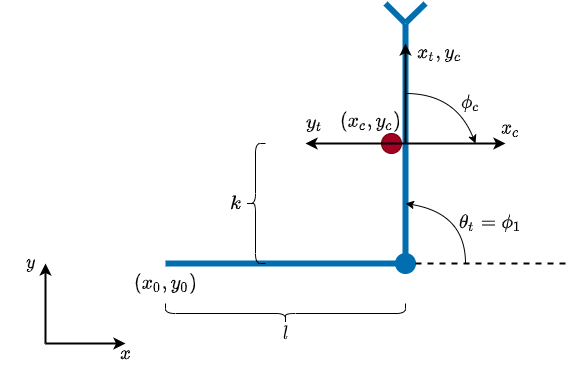
\includegraphics[width=0.9\textwidth]{figures/theory/example_2link.png}
    \caption{Model of 2-link snake robot}
    \label{fig:ex_2link}
\end{figure}

The joint variables are given by

\begin{equation}
    \mathbf{q} =
    \begin{bmatrix}
        \phi_0 & \phi_1 & x_0 & y_0 & k & \phi_c
    \end{bmatrix}^T \in \mathcal{R}^5.
\end{equation}
\\
The task coordinates by the contact point are given by

\begin{equation}
    \mathbf{r}_t = 
    \begin{bmatrix}
        x_c & y_c & \theta_t
    \end{bmatrix}^T \in \mathcal{R}^3,
\end{equation}
\\
where $\theta_t$ in the given configuration is the sum of the two joint angles $\phi_0$ and $\phi_1$. Furthermore, the constraint coordinates, which should always remain constant, are given by

\begin{equation}
    \mathbf{r}_c = 
    \begin{bmatrix}
        x_c & y_c & \theta_c
    \end{bmatrix}^T \in \mathcal{R}^3,
\end{equation}
\\
where $\theta_c$ is the angle of the obstacle point coordinate system in the base frame. This angle should always be zero, as can be seen from Figure \ref{fig:ex_2link}. It should be noted that the origin of the two frames, described by $(x_c, y_c)$, is the same. This is a result of the contact point and obstacle being modeled as a single point.

Lastly, the velocities and forces represented in the task frame (visualized in Figure \ref{fig:ex_2link} as $(x_t, y_t)$) are 

\begin{equation}
    \mathbf{v} =
    \begin{bmatrix}
        v_x & v_y
    \end{bmatrix}^T \in \mathcal{R}^2,
\end{equation}

\begin{equation}
    \mathbf{f} =
    \begin{bmatrix}
        f_x & f_y
    \end{bmatrix}^T \in \mathcal{R}^2.
\end{equation}
\\

\subsubsection{Dynamics}

The dynamics of this robot can be found using the Euler-Lagrange method described in \ref{sec:dyn}.
The position and velocities of the middle of the links in the base frame are

\begin{equation}
    \begin{split}
        p_0 &=
        \begin{bmatrix}
            x_0 + l/2 cos(\phi_0)\\
            y_0 + l/2 sin(\phi_0)
        \end{bmatrix}, \\
        p_1 &=
        \begin{bmatrix}
            x_0 + l cos(\phi_0) + l/2 cos(\phi_0+ \phi_1)\\
            y_0 + l sin(\phi_0) + l/2 sin(\phi_0+\phi_1)
        \end{bmatrix},
    \end{split}
\end{equation}

\begin{equation}
    \begin{split}
        \dot{p}_0 &=
        \begin{bmatrix}
            \dot{x_0} - l/2 \dot{\phi_0} sin(\phi_0)\\
            \dot{y_0} + l/2 \dot{\phi_0} cos(\phi_0)
        \end{bmatrix}, \\
        \dot{p}_1 &=
        \begin{bmatrix}
            \dot{x_0} - l \dot{\phi_0} sin(\phi_0) - l/2 (\dot{\phi}_0 +\dot{\phi}_1) sin(\phi_0+\phi_1)\\
            \dot{y_0} + l \dot{\phi_0} cos(\phi_0) + l/2 (\dot{\phi}_0 +\dot{\phi}_1) cos(\phi_0+\phi_1)
        \end{bmatrix}.
    \end{split}
\end{equation}
\\
The Lagrangian and the dynamical equations can now be calculated from (\ref{eq:ex_dyn1}) and (\ref{eq:ex_dyn2}), where $I = (1/12)ml^2 = 1/12$.

\begin{equation}\label{eq:ex_dyn1}
    \begin{split}
        L &= K_{translational,0} + K_{rotational,0} + K_{translational,1} + K_{rotational,1}\\
        &= \frac{1}{2} m \dot{p}_0^2 + \frac{1}{2}I\dot{\phi_0}^2 + \frac{1}{2} m \dot{p}_1^2 + \frac{1}{2}I\dot{\phi_1}^2
    \end{split}
\end{equation}
\\
\begin{equation}\label{eq:ex_dyn2}
    \boldsymbol{\tau} = \frac{d}{dt} \frac{\partial L}{\partial \dot{\mathbf{q}}} - \frac{\partial L}{\partial \mathbf{q}}
\end{equation}
\\
Inserting the values for the constants $m$ and $l$ and comparing the result to the form given in (\ref{eq:eom}) gives the inertia and Coriolis matrix in (\ref{eq:ex_inertia}) and (\ref{eq:ex_coriolis}) respectively. The trigonometric functions are abbreviated to $s_0 = sin(\phi_0)$, $s_1 = sin(\phi_1)$, $c_0 = cos(\phi_0)$, $c_1 = cos(\phi_1)$, $s_{01} = sin(\phi_0+\phi_1)$ and $c_{01} = cos(\phi_0+\phi_1)$.

\begin{equation}\label{eq:ex_inertia}
    \mathbf{M(q)} = 
    \begin{bmatrix}
        c_1+\frac{5}{3} & \frac{c_1}{2} + \frac{1}{3} & -\frac{s_{01}}{2} - \frac{3s_0}{2} & \frac{c_{01}}{2} + \frac{3c_0}{2} & 0 & 0 \\
        \frac{c_1}{2}+\frac{1}{3} & \frac{1}{3} & -\frac{s_{01}}{2} & \frac{c_{01}}{2} & 0 & 0 \\
        -\frac{s_{01}}{2}- \frac{3s_0}{2} & -\frac{s_{01}}{2} & 2 & 0 & 0 & 0 \\
        \frac{c_{01}}{2}+ \frac{3c_0}{2} & \frac{c_{01}}{2} & 0 & 2 & 0 & 0 \\
        0 & 0 & 0 & 0 & 0  & 0 \\
        0 & 0 & 0 & 0 & 0  & 0
    \end{bmatrix}
\end{equation}

\begin{equation}\label{eq:ex_coriolis}
    \mathbf{C(q, \dot{q})} = 
    \begin{bmatrix}
        -\frac{\dot{\phi}_1 s_1 (2\dot{\phi}_0+ \dot{\phi}_1)}{2} \\
        \frac{\dot{\phi}_0^2 s_1}{2} \\
        -\frac{3 \dot{\phi}_0^2 c_1}{2} - \frac{\dot{\phi}_0^2 c_{01}}{2} - \frac{\dot{\phi}_1^2 c_{01}}{2} - \dot{\phi}_0 \dot{\phi}_1 c_{01} \\
        -\frac{3 \dot{\phi}_0^2 s_1}{2} - \frac{\dot{\phi}_0^2 s_{01}}{2} - \frac{\dot{\phi}_1^2 s_{01}}{2} - \dot{\phi}_0 \dot{\phi}_1 s_{01} \\
        0 \\ 0
    \end{bmatrix}
\end{equation}
\\
Inserting the given angles significantly simplifies the matrices to

\begin{equation}
    \mathbf{M} = 
    \begin{bmatrix}
        5/3 & 1/3 & -1/2 & 3/2 & 0& 0 \\
        1/3 & 1/3 & -1/2 & 0 & 0 & 0\\
        -1/2 & -1/2 & 2 & 0 & 0 & 0\\
        3/2 & 0 & 0 & 2 & 0 & 0\\
        0 & 0 & 0 & 0 & 0 & 0\\
        0 & 0 & 0 & 0 & 0 & 0
    \end{bmatrix}
\end{equation}

\begin{equation}
    \mathbf{C(\dot{q})} = 
    \begin{bmatrix}
        -(\dot{\phi}_1 (2\dot{\phi}_0+ \dot{\phi}_1))/2 \\
        \dot{\phi}_0^2/2 \\
        0 \\
        -3 \dot{\phi}_0^2/2 - \dot{\phi}_0^2/2 - \dot{\phi}_1^2/2 - \dot{\phi}_0 \dot{\phi}_1 \\
        0 \\ 0
    \end{bmatrix}.
\end{equation}

\subsubsection{Constraints}

The single obstacle present in this example stands for the single constraint on the snake robot. 
From \ref{subsec:DHPFC} it is known that the constraint is on the velocity of the contact point normal to the link in contact. This velocity is here given as

\begin{equation}
    v_y = - sin(\theta_t) \dot{x}_c + cos(\theta_t) \dot{y}_c
\end{equation}
\\
In order for the link to both stick to the obstacle and not penetrate it, the velocity $v_y$ should be zero. This constraint is put on the form in (\ref{eq:hpfc:derhypsurf}) and the given angles are inserted.

\begin{equation}\label{eq:ex_EF}
    \mathbf{E}_F = 
    \begin{bmatrix}
        - sin(\theta_t) & cos(\theta_t) & 0
    \end{bmatrix}
    =
    \begin{bmatrix}
        - 1 & 0 & 0
    \end{bmatrix}
\end{equation}
\\
The derivative of (\ref{eq:ex_EF}) is
\begin{equation}\label{eq:ex_EFd}
    \mathbf{\dot{E}}_F = 
    \begin{bmatrix}
        -cos(\theta_t) \dot{\theta}_t & - sin(\theta_t) \dot{\theta}_t & 0
    \end{bmatrix}
    \begin{bmatrix}
        0 & -\dot{\theta}_t & 0
    \end{bmatrix}.
\end{equation}
\\
Inserting (\ref{eq:ex_EFd}) into (\ref{eq:dhpfc_arf}) gives
\begin{equation}
    a_{rF} = -\dot{\theta}_t \dot{y}_c.
\end{equation}
\\
It is however known that the obstacle itself cannot move. This, together with the obstacle being modeled as a point, results in the velocity of the contact point being zero at all times. Thus $a_{rF}=0$.

(\ref{eq:dhpfc_EPi}) and (\ref{eq:dhpfc_E}) give
\begin{equation}
    \mathbf{E}_P = 
    \begin{bmatrix}
        cos(\theta_t) & sin(\theta_t) & 0 \\
        0 & 0 & 1
    \end{bmatrix}=
    \begin{bmatrix}
        0 & 1 & 0 \\
        0 & 0 & 1
    \end{bmatrix},
\end{equation}
\begin{equation}
    \mathbf{E}=
    \begin{bmatrix}
        0 & 1 & 0 \\
        0 & 0 & 1 \\
        -1 & 0 & 0
    \end{bmatrix}.
\end{equation}
\\
The task coordinates can be expressed as
\begin{equation}
    \mathbf{r}_t =
    \begin{bmatrix}
        x_0 + l cos(\phi_0) + k cos(\phi_0+\phi_1)\\
        y_0 + l sin(\phi_0) + k sin(\phi_0+\phi_1)\\
        \phi_0+\phi_1
    \end{bmatrix}.
\end{equation}
\\
The corresponding Jacobian an its derivative can thus be calculated to
\begin{equation}
    \begin{split}
        \mathbf{J}_t&=
        \begin{bmatrix}
            -l s_0 - k s_{01} & - k s_{01} & 1 & 0 & c_{01} & 0 \\
            l c_0 + k c_{01} & k c_{01} & 0 & 1 & s_{01} & 0 \\
            1 & 1 & 0 & 0 & 0 & 0
        \end{bmatrix}\\&=
        \begin{bmatrix}
            - k & - k & 1 & 0 & 0 & 0 \\
            1 &0 & 0 & 1 & 1 & 0 \\
            1 & 1 & 0 & 0 & 0 & 0
        \end{bmatrix},
    \end{split}
\end{equation}
\begin{equation}\label{eq:ex_Jd}
    \begin{split}
        \mathbf{\dot{J}}_t&=
        \begin{bmatrix}
            - \dot{k} s_{01} -l \dot{\phi}_0c_0 -k c_{01}(\dot{\phi_0}+\dot{\phi_1}) & -\dot{k} s_{01}-k c_{01}(\dot{\phi_0}+\dot{\phi_1}) & 0 & 0 & -s_{01}(\dot{\phi_0}+\dot{\phi_1})  & 0\\
            \dot{k} c_{01} -l \dot{\phi}_0s_0 -k s_{01}(\dot{\phi_0}+\dot{\phi_1}) & \dot{k} c_{01}-k s_{01}(\dot{\phi_0}+\dot{\phi_1}) & 0 & 0 & c_{01}(\dot{\phi_0}+\dot{\phi_1}) & 0 \\
            0 & 0 & 0 & 0 & 0 & 0
        \end{bmatrix}\\&=
        \begin{bmatrix}
            - \dot{k} -\dot{\phi}_0 & -\dot{k} & 0 & 0 & -(\dot{\phi_0}+\dot{\phi_1}) & 0 \\
            -\dot{k}(\dot{\phi_0}+\dot{\phi_1}) & -\dot{k}(\dot{\phi_0}+\dot{\phi_1}) & 0 & 0 & 0 & 0\\
            0 & 0 & 0 & 0 & 0 & 0
        \end{bmatrix}.
    \end{split}
\end{equation}
\\
Inserting (\ref{eq:ex_Jd}) into (\ref{eq:dhpfc_aq}) gives
\begin{equation}
    \mathbf{a}_q =
    \begin{bmatrix}
            - (\dot{k} +\dot{\phi}_0)\dot{\phi}_0 -\dot{k} \dot{\phi}_1 -(\dot{\phi_0}+\dot{\phi_1})\dot{k} \\
            -\dot{k}(\dot{\phi_0}+\dot{\phi_1})\dot{\phi}_0 -\dot{k}(\dot{\phi_0}+\dot{\phi_1})\dot{\phi}_1 \\
            0
        \end{bmatrix}.
\end{equation}

\subsubsection{Calculation of the control torque}

All matrices necessary to derive the control torque are now defined. To make the calculation of the torque even simpler, the static case where all velocities are zero is considered. The result is calculated using (\ref{eq:dhpfc_tau_c})-(\ref{eq:dhpfc_qddd}) and a desired force $f_F = 1 N$ and desired acceleration $\ddot{\mathbf{r}}_d = [0, 0, 1 rad/s^2]^T$. \hl{Quite fast rotation and light force?}

\begin{equation}
    \mathbf{\ddot{q}}_d =
    \begin{bmatrix}
        0 & \frac{1}{5} & \frac{2}{5}\\
        0 & -\frac{1}{5} & \frac{3}{5}\\
        1 & 0 & k \\
        0 & \frac{2}{5} & -\frac{1}{5}\\
        0 & \frac{2}{5} & -\frac{1}{5} \\
        0 & 0 & 0
    \end{bmatrix}\left\{
    \begin{bmatrix}
        0 & 0 & -1\\
        1 & 0 & 0\\
        0 & 1 & 0
    \end{bmatrix}
    \begin{bmatrix}
        0\\   1\\   0
    \end{bmatrix}-
    \begin{bmatrix}
        0\\   0\\   0
    \end{bmatrix}\right\}=
    \begin{bmatrix}
        \frac{2}{5}\\
        \frac{3}{5}\\
        k \\
        -\frac{1}{5}\\
        -\frac{1}{5} \\
        0
    \end{bmatrix}
\end{equation}
\\
The distance $k$ from the joint to the obstacle is chosen to be $1/2 m$.
\begin{equation}
    \boldsymbol{\tau}_P = 
    \begin{bmatrix}
        5/3 & 1/3 & -1/2 & 3/2 & 0 & 0 \\
        1/3 & 1/3 & -1/2 & 0 & 0 & 0 \\
        -1/2 & -1/2 & 2 & 0 & 0 & 0 \\
        3/2 & 0 & 0 & 2 & 0 & 0 \\
        0 & 0 & 0 & 0 & 0  & 0\\
        0 & 0 & 0 & 0 & 0  & 0
    \end{bmatrix}
    \begin{bmatrix}
        2/5\\
        3/5\\
        k \\
        -1/5\\
        -1/5\\0
    \end{bmatrix}=
    \begin{bmatrix}
        0.3167\\
        0.0833\\
        0.5000 \\
        0.2000\\
        0\\0
    \end{bmatrix}
\end{equation}

\begin{equation}
    \boldsymbol{\tau}_F = 
    \begin{bmatrix}
       -k & 1 & 1\\
       -k & 0 & 1\\
       1 & 0 & 0\\
       0 & 1 & 0\\
       0 & 1 & 0 \\
       0 & 0 & 0
    \end{bmatrix}
    \begin{bmatrix}
        -1 \\ 0 \\ 0
    \end{bmatrix}=
    \begin{bmatrix}
       0.5000\\
       0.5000\\
       -1.000\\
       0.000\\
       0.000\\ 0
    \end{bmatrix}
\end{equation}

\begin{equation}
    \boldsymbol{\tau}_c =
    \begin{bmatrix}
        0.8167 & 0.5833 & -0.5000 & 0.2000 & 0.000 & 0.000
    \end{bmatrix}^T
\end{equation}

\hl{Discuss this result. The torques to the translational positions cannot be applied. Is this what the servo feedback thing is for?? only tau 1 can really be applied. k ends up being a free variable!}

%%%%%%%%%%%%%%%%%%%%%%%%%%%%%%%%%%%%%%%%%%%%%%%%%%%%%%%%%%%%%%%%%%%%%%%%%%%%%%%%%%%%%%%%%%%%%
%%%%%%%%%%%%%%%%%%%%%%%%%%%%%%%%%%%%%%%%%%%%%%%%%%%%%%%%%%%%%%%%%%%%%%%%%%%%%%%%%%%%%%%%%%%%%
%%%%%%%%%%%%%%%%%%%%%%%%%%%%%%%%%%%%%%%%%%%%%%%%%%%%%%%%%%%%%%%%%%%%%%%%%%%%%%%%%%%%%%%%%%%%%

